%!TEX output_directory = aux

\documentclass[11pt]{article}

\usepackage[english]{babel}

% ---- FONT & MICROTYPOGRAPHY ----
\usepackage[utf8]{inputenc}
\usepackage[T1]{fontenc}
\usepackage{microtype}
\usepackage{moresize}

% ---- FORMATTING ----
\usepackage{csquotes,textcase,xspace}

% ---- PAGE LAYOUT ----
\usepackage{geometry}
\geometry{top=2.5cm,bottom=2cm,inner=2cm,outer=2cm,footnotesep=7mm plus 4pt minus 4pt}
\usepackage{setspace}
\setstretch{1.1}

% ---- GRAPHIQUE ----
\usepackage{graphicx}
\usepackage{xcolor}
\usepackage[font=small,labelfont=bf,labelsep=space]{caption}
\usepackage{subfigure}
\captionsetup{width=0.9\textwidth,font={small,stretch=1.1}}
\addto\captionsenglish{\renewcommand{\figurename}{Fig.}}
\addto\captionsenglish{\renewcommand{\tablename}{Tab.}}
\definecolor{JoliBleu}{rgb}{0,0.55,0.55}
\definecolor{JoliVert}{rgb}{0.15,0.6,0}
\definecolor{JoliRouge}{rgb}{0.86,0.08,0}
\definecolor{JoliJaune}{rgb}{1,0.75,0}
\definecolor{JoliGris}{rgb}{0.52,0.52,0.51}
\definecolor{myblue}{RGB}{26, 77, 116}
\definecolor{myorange}{RGB}{181, 116, 30}
\definecolor{mydarkorange}{RGB}{166, 88, 0}
\definecolor{mygreen}{RGB}{21, 124, 80}
\definecolor{myblack}{RGB}{43, 65, 82}
\definecolor{myred}{rgb}{0.5, 0.0, 0.13}

% ---- SECTIONING ----
\usepackage{titlesec}
\titleformat{\section}[block]{\Large\boldmath\bfseries}{\thesection}{1em}{}
\titleformat{\subsection}[block]{\large\boldmath\bfseries}{\thesubsection}{0.5em}{}
\usepackage{appendix}
\renewcommand{\setthesection}{\Alph{section}}
\renewcommand{\restoreapp}{}
\makeatletter
\renewcommand{\theequation}{\thesection.\arabic{equation}}
\@addtoreset{equation}{section}
\makeatother

% ---- FOOTERS HEADERS ----
\usepackage[bottom]{footmisc}
\usepackage{fancyhdr}

% ---- TABLE OF CONTENTS ----
\usepackage{titletoc}
\setcounter{tocdepth}{3}

% ---- BIBLIOGRAPHY ----
\usepackage[nosort]{cite}
\bibliographystyle{JHEP}
\newcommand{\eprint}[1]{{\href{http://arxiv.org/abs/#1}{\texttt{[#1]}}}}
\newcommand{\eprintN}[1]{{\href{http://arxiv.org/abs/#1}{\texttt{#1 [hep-th]}}}}
\newcommand{\doi}[2]{\href{http://dx.doi.org/#2}{#1}}

% ---- HYPER REF ----
\usepackage{hyperref}
\hypersetup{colorlinks=true,
        pdfstartview=FitV,
        linkcolor= mydarkorange,
        citecolor= mydarkorange,
        urlcolor= JoliGris!60!black,
        hypertexnames=false,
        linktoc=page}

% ---- TIKZ ----
\usepackage{tikz}
\usetikzlibrary{calc}

% ---- MATHS ----
\usepackage{amsmath,amssymb,amsfonts,dsfont}
\usepackage{mathrsfs}
\usepackage{physics}
\usepackage{ytableau}
\ytableausetup{boxsize=1.1em,centertableaux}
\usepackage{stmaryrd}
\usepackage{nicefrac}
\allowdisplaybreaks[1]
% \usepackage{bbold}
\usepackage{cases}
\usepackage{bm}
\usepackage{bbm}

% ---- TABLES ----
\usepackage{multirow}
\usepackage{booktabs}
\usepackage{pdflscape}
\usepackage{array}
\usepackage{arydshln}

% ---- ENUMERATION ----
\usepackage[shortlabels]{enumitem}

% ---- MATHS COMMANDS ----
\newcommand{\A}{\ensuremath{\mathcal{A}}\xspace}
\newcommand{\F}{\ensuremath{\mathcal{F}}\xspace}
\renewcommand{\H}{\ensuremath{\mathcal{H}}\xspace}
\newcommand{\M}{\ensuremath{\mathcal{M}}\xspace}
\renewcommand{\P}{\ensuremath{\mathcal{P}}\xspace}
\newcommand{\J}{\ensuremath{\mathcal{J}}\xspace}
\renewcommand{\d}{\ensuremath{\mathrm{d}}\xspace}
\renewcommand{\H}{\ensuremath{\mathcal{H}}\xspace}
\newcommand{\SO}{\ensuremath{\mathrm{SO}}\xspace}
\renewcommand{\O}{\ensuremath{\mathrm{O}}\xspace}
\newcommand{\SL}{\ensuremath{\mathrm{SL}}\xspace}
\newcommand{\Odd}{\ensuremath{\mathrm{O}(d,d)}\xspace}
\newcommand{\odd}{\ensuremath{\mathfrak{o}(d,d)}\xspace}
\renewcommand{\Tr}[1]{\ensuremath{\mathrm{Tr}\left(#1\right)}\xspace}
\newcommand{\vol}{{\,\rm vol}}
\def\sst#1{{\scriptscriptstyle #1}}


\def\0{{\sst{(0)}}}
\def\1{{\sst{(1)}}}
\def\2{{\sst{(2)}}}
\def\3{{\sst{(3)}}}
\def\4{{\sst{(4)}}}
\def\5{{\sst{(5)}}}
\def\6{{\sst{(6)}}}
\def\7{{\sst{(7)}}}
\def\8{{\sst{(8)}}}

\newcommand{\be}{\begin{equation}}
\newcommand{\ee}{\end{equation}}

% ---- COMMENTS ----
\usepackage[subfigure]{tocloft}		
\newcommand{\listnotetitle}{\Large List of Notes}
\newlistof{notes}{nt}{\listnotetitle}
\newcommand{\notelist}[1]{%
	\refstepcounter{notes}
	\addcontentsline{nt}{notes}
	{\protect\numberline{\thenotes}#1}
}

\newcommand{\note}[1]{\notelist{#1}\marginpar{\parbox{\marginparwidth}{\boldmath $\Longleftarrow$}}{\boldmath\bfseries Note: #1}}


% ---- TITLE PAGE ----
\usepackage[affil-it]{authblk}
\def\preprint{}

\makeatletter
\def\@maketitle{%
  \newpage
  \null\hfill\texttt{\preprint}
  \vskip 4em%
  \begin{center}%
  \let \footnote \thanks
    {\LARGE\bfseries \@title \par}%
    \vskip 2.5em%
    {\large
      \lineskip .5em%
      \begin{center}
        \begin{minipage}{0.95\textwidth}
            \begin{tabular}[t]{c}%
            \@author
            \end{tabular}
        \end{minipage}    
      \end{center}\par}%
    \vskip 1em%
    {\large \@date}%
  \end{center}%
  \par
  \vskip 1.5em}
\makeatother

\renewcommand\Authands{ and }

\title{Notes on conformal manifolds}
\author{}



%%%%%%%%%%%%%%%%%%%%%%%%%%%%%%%%%%
%%%%%%%%%%%%%%%%%%%%%%%%%%%%%%%%%%


\begin{document}

\maketitle


Workflow as of \today:
\begin{enumerate}
	\item Generate larger clouds of points for the 7- and 13-param potentials (Gabriel).
	\item For these two models, get statistics of autoencoders for several attempts per dimension of latent layer (Bastien).
	\item Go up to full 32-param SO(8,4) potential.
\end{enumerate}

\tableofcontents


%%%%%%%%%%%%%%
%%%%%%%%%%%%%%
\section{Comments on Flat Directions and $n$-Hessians} \label{sec: hessians}
%%%%%%%%%%%%%%

Given a real function $V: M \rightarrow \mathbb R$, its critical points are defined as the zeroes of the gradient
%
\begin{equation}
	x^*: H_{m}(x^*)\equiv\partial_mV\big\vert_{x^*}=0\,,
\end{equation}
%
with the $n$-Hessian of $V(x)$ defined as
%
\begin{equation}
	H_{m_1\dots m_n}\equiv\partial_{m_1}\dots\partial_{m_n}V\,.
\end{equation}
%

Flat directions around the critical point $x^*$ are curves $\phi: I\rightarrow M$ such that
%
\begin{equation}	\label{eq: flatdef}
	H_{m}(\phi(t))=0\,,	\qquad\text{with}\quad
	\phi(0)=x^*\,.
\end{equation}
%
Close to $x^*$, the curve can be expanded as
%
\begin{equation}	\label{eq: phiSeries}
	\phi(t)=x^*+\sum_{k=1}^{\infty}\tfrac1{k!}\xi_k\, t^k\,, \qquad\text{with}\quad
	\xi_k=\frac{d^k\phi}{dt^k}\Big\vert_{x^*}\,,
\end{equation}
%
and, accordingly,
%
\begin{equation}
	\begin{aligned}
		H_{m}(\phi(t))&=\sum_{k=1}^{\infty}H_{mn_1\dots n_k}\sum_{a\in\lambda_k}t^{\sum_i^{\vert a\vert}i a_i}\bigg[\prod_{i=1}^{\vert a\vert}\frac1{a_i!}\frac{1}{\big(i!\big)^{a_i}}\xi_i^{\otimes a_i}\bigg]^{n_1\dots n_k}\,,
	\end{aligned}
\end{equation}
%
with all the $n$-Hessians on the right-hand side evaluated at $x^*$. Here, $\lambda_k$ denotes the integer partitions of $k$ (e.g. $\lambda_3=\{(3),(2,1),(1,1,1)\}$), $\vert a\vert$ is the number of elements of a specific partition $a\in\lambda_k$ (e.g. $\vert(2,1)\vert=2$ and $\vert(1,1,1)\vert=3$), and $a_i$ each of its elements. Equation \eqref{eq: flatdef} needs to be satisfied at every order in $t$, and therefore the existence of flat directions amounts to the existence solutions of the system
%
\begin{equation}	\label{eq: flateqnsAll}
	O(t^p):\quad\sum_{\{a_i\}}H_{mn_1\dots n_{k}}\prod_i^{p}\bigg[\frac1{a_i!}\frac1{\big(i!\big)^{a_i}}\xi_i^{\otimes a_i}\bigg]^{n_1\dots n_k}=0\,,
\end{equation}
%
with the set of coefficients $\{a_i\}$ determined as
%
\begin{equation}	\label{eq: as}
	\sum_i^{p}i a_i=p\,, 	\qquad
	a_i\in \mathbb{N}\,,
\end{equation}
%
and $k$ in \eqref{eq: flateqnsAll} a shorthand for $k=\sum_i^p a_i$ for the solutions of \eqref{eq: as}.
For lowest $p$, this is \note{Can map to CFT $n$-point functions à la Bertolini?}
%
\begin{equation}	\label{eq: flateqns}
	\begin{aligned}
		0&=H_{mn}\xi_1^n\,,		\\[5pt]
		0&=H_{mn}\xi_2^n+H_{mnp}\xi_1^n\xi_1^p\,,	\\[5pt]
		0&=H_{mn}\xi_3^n+3H_{mnp}\xi_2^n\xi_1^p+H_{mnpq}\xi_1^n\xi_1^p\xi_1^q\,,	\\[5pt]
		0&=H_{mn}\xi_4^n+3H_{mnp}\xi_2^n\xi_2^p+4H_{mnp}\xi_3^n\xi_1^p+6H_{mnpq}\xi_2^n\xi_1^p\xi_1^q+H_{mnpqr}\xi_1^n\xi_1^p\xi_1^q\xi_1^r\,,	\\[5pt]
		&\dots
	\end{aligned}
\end{equation}
%

Note that the non-linearity of \eqref{eq: flateqns} in the expansion coefficients of $\phi(t)$ implies that the number of flat directions is not easily related to the dimension of the null space of the 2-Hessian at $x^*$ (i.e. the number of massless scalars if $V$ is the scalar potential). A necessary condition for \eqref{eq: flateqnsAll} to have a solution is
%
\begin{equation}
	\det H_{mn}=0\,,		\\[5pt]
\end{equation}
%
but there can be more flat directions than zero eigenvalues and vice versa. These features will be studied in the following.

%%%%%%%%%%%%%%
\subsection{Flat flat directions} \label{sec: FFC}
%%%%%%%%%%%%%%


When flat directions can be given as straight lines $\phi(t)=x^*+\xi t$ for constant $\xi$, the set of equations \eqref{eq: flateqns} simplifies to the condition $\xi\in K_k$ for all $n\geq1$, with the kernels defined as
%
\begin{equation}	\label{eq: flatness}
	K_k=\{\xi: \xi^{n_1}\dots\xi^{n_{k}}H_{mn_1\dots n_{k}}(x^*)=0\}\,,	\qquad \forall n\geq1\,.
\end{equation}
%
This condition is required for $\partial_mV$ to be constant along the integral curve of $\xi^m$, since
%
\begin{equation}
	\begin{aligned}
		\xi^{n_k}\partial_{n_k}\big(\xi^{n_1}\dots\xi^{n_{k-1}}H_{mn_1\dots n_{k-1}}\big)\big\vert_{x^*}
		=\xi^{n_1}\dots\xi^{n_{k}}H_{mn_1\dots n_{k}}(x^*)
	\end{aligned}
\end{equation}
%
must hold for all $k\geq1$.

Two functions that have flat flat directions and exhibit the subtleties mentioned before are given by
%
\begin{equation}	\label{eq: flatflat}
	V_1(x,y)=x^4(1+y^2)\,,		\qquad\text{and}\qquad
	V_3(x,y)=y^2(x^2-3y^2)^2\,,
\end{equation}
%
which are plotted in Fig.~\ref{fig: flatflat}.
%
\begin{figure}
	\centering
	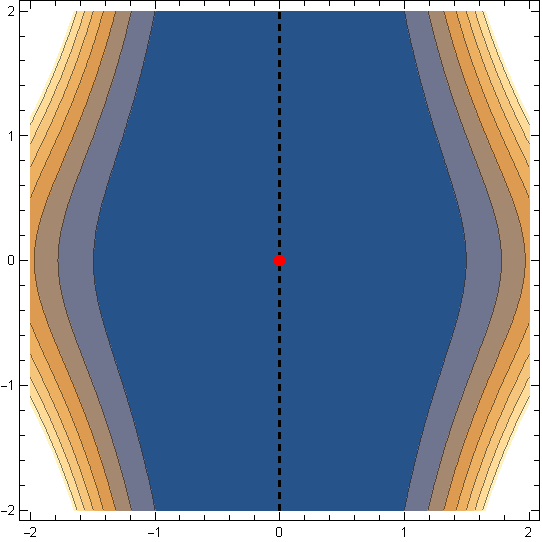
\includegraphics[width=0.4\textwidth]{Figures/V1.pdf}
	\qquad
	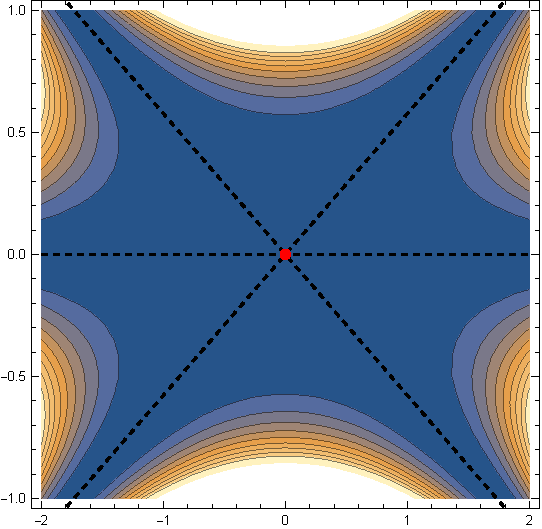
\includegraphics[width=0.4\textwidth]{Figures/V3.pdf}
	\caption{Contour plots for the potentials $V_1$ (left) and $V_3$ (right) in \eqref{eq: flatflat} with flat directions and $x^*=0$ locus superimposed.}
	\label{fig: flatflat}
\end{figure}
%
In both cases, the 2-Hessian vanishes identically at $x^*=0$, but $V_1$ only has one flat direction given by $(x,y)=(0,\zeta)$, whereas $V_3$ has three independent flat curves:
%
\begin{equation}
	(x,y)=(0,\, \zeta_1)\,,	\qquad
	(x,y)=(\sqrt3\,\zeta_2,\, \zeta_2)\,,	\qquad
	(x,y)=(-\sqrt3\,\zeta_3,\, \zeta_3)\,.
\end{equation}
%

\note{How is the second compatible with the standard holography lore? Can this type of potentials arise in consistent truncations?}

\note{We should remark that conformal manifolds are not smooth manifolds in general, but algebraic varieties. Apparently, people doing quivers know this [look at papers by Hanany]}

%%%%%%%%%%%%%%
\subsection{Curved flat directions} \label{sec: FCL}
%%%%%%%%%%%%%%

(alternative name: curved flat curves)

The condition \eqref{eq: flatness} does not capture curves with a non-linear dependence on $t$. For instance,
%
\begin{equation}	\label{eq: Vcurved}
	V(x,y)=x^2(x^2-3y^4)^2
\end{equation}
%
has flat directions
%
\begin{equation}	\label{eq: curvedcurves}
	(x,y)=(0,\, \zeta_1)\,,	\qquad
	(x,y)=(\sqrt3\,\zeta_2^2,\, \zeta_2)\,,	\qquad
	(x,y)=(-\sqrt3\,\zeta_3^2,\, \zeta_3)\,,
\end{equation}
%
of which only the first is captured by \eqref{eq: flatness}. For the other two, the higher order terms in \eqref{eq: flateqnsAll} also contribute. To gauge-fix the reparameterisation invariance of \eqref{eq: flatdef}, we demand without loss of generality that the lowest non-vanishing term in \eqref{eq: phiSeries} is linear in $t$.  Doing so, \eqref{eq: flateqnsAll} yields \eqref{eq: curvedcurves} unambiguously. We note that for \eqref{eq: Vcurved} the first non-trivial equation arises at order $O(t^5)$, the following at $O(t^{10})$, and from then on we get a condition on every level.

This method has been checked with three other functions with flat directions:
%
\begin{equation}
	\begin{aligned}
		V(x,y)&=(y-\cos x)^2\,,	\\[5pt]
		V(x,y)&=(x^2+y^2-1)^2\,,	\\[5pt]
		V(x,y)&=x^2(x^2+y^2-1)^2\,,
	\end{aligned}
\end{equation}
%
recovering the analytic result in all instances and converging more quickly than for \eqref{eq: Vcurved} (as their series have non-zero contributions at lower orders).

\note{The distinction between the different curves in \eqref{eq: curvedcurves} disappears at linear level, and this is very reminiscent of the TsT vs Wilson loop families in \cite{Eloy:2024lwn}.}


%
\begin{figure}
	\centering
	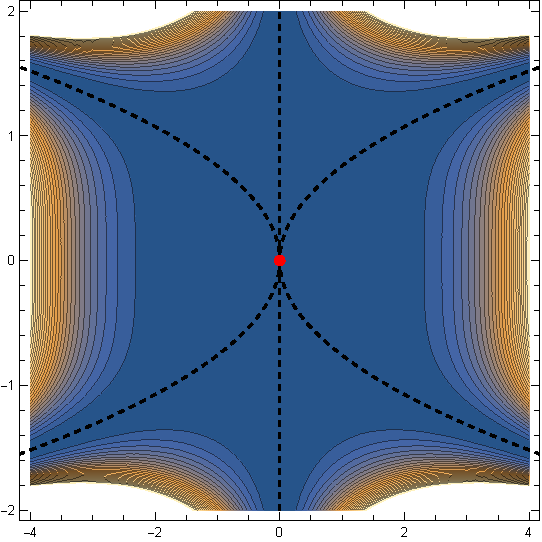
\includegraphics[width=0.5\textwidth]{Figures/V3curved.pdf}
	\caption{Contour plot for the potential in \eqref{eq: Vcurved} with flat directions in \eqref{eq: curvedcurves} and $x^*=0$ locus superimposed.}
	\label{fig: curvedflat}
\end{figure}
%


%%%%%%%%%%%%%%
\section{Machine Learning Approach} \label{sec: MLapproach}
%%%%%%%%%%%%%%

In the following, we obtain and analyse numerically the critical points of different functions $V: \mathbb{R}^n\rightarrow\mathbb{R}$. 
In this approach, a cloud of points $x_i^m$, $m\in\llbracket1,n\rrbracket$ and $i\in\llbracket1,N\rrbracket$,
is generated so that the loss function
%
\begin{equation}	\label{eq: loss_cloud}
	L_{V}=\sum_i^N\vert \nabla_m V(x_i)\vert^2
\end{equation}
%
is minimised. 
For this minimisation, we have employed an protocol based on the \texttt{TensorFlow} Adam optimiser 
which restarts the optimiser with the initial learning rate after a specified number of epochs until a specified loss value is attained.
Afterwards and until the pre-determined number of epochs is reached, the learning rate decreases by a factor 10 every few epochs 
(in the \texttt{grad\_descent\_module.py} package, the original learning rate us used by default for the first 2500 epochs with restarts every 200
steps, and then updated every 2500 steps. These parameters need to be adapted to the potential under consideration).

The structure of the resulting cloud of points minimising \eqref{eq: loss_cloud} is subseqently learnt using
autoencoders (AEs), which are non-linear endomorphisms constructed via a neural network with an intermediate layer
of dimension $\ell < n$, as schematically depicted in figure~\ref{fig: AE_notation}. 
%
\begin{figure}
	\centering
	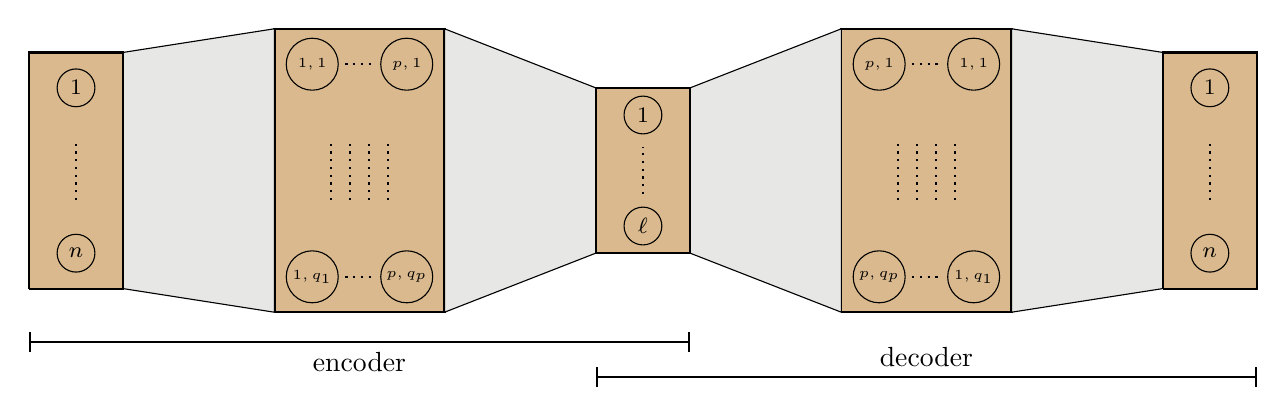
\begin{tikzpicture}[scale=3]
		\def\xlim{.2}
		\def\ylim{0.5}
		\def\dist{1.2}	% distance between rectangles from center to center

		% Latent layer
		\draw[thick,fill=myorange!50] (-\xlim,-0.7*\ylim) -- (\xlim,-0.7*\ylim) -- (\xlim,0.7*\ylim) -- (-\xlim,0.7*\ylim)-- (-\xlim,-0.7*\ylim);
		\draw (0,0.47*\ylim) circle [radius = 0.4*\xlim] node {\footnotesize{$1$}};
		\draw (0,-0.47*\ylim) circle [radius = 0.4*\xlim] node {\footnotesize{$\ell$}};
		\draw[thick, dotted] (0,-0.2*\ylim) -- (0,0.2*\ylim);
		
		% Hidden layers left
		\draw[thick,fill=myorange!50] (-1.8*\xlim-\dist,-1.2*\ylim) -- (1.8*\xlim-\dist,-1.2*\ylim) -- (1.8*\xlim-\dist,1.2*\ylim) -- (-1.8*\xlim-\dist,1.2*\ylim)-- (-1.8*\xlim-\dist,-1.2*\ylim);
		
		\draw (-\dist-1.0*\xlim,0.9*\ylim) circle [radius = 0.55*\xlim] node {\tiny{$1,1$}};
		\draw (-\dist-1.0*\xlim,-0.9*\ylim) circle [radius = 0.55*\xlim] node {\tiny{$1,q_1$}};
		\draw (-\dist+1.0*\xlim,0.9*\ylim) circle [radius = 0.55*\xlim] node {\tiny{$p,1$}};
		\draw (-\dist+1.0*\xlim,-0.9*\ylim) circle [radius = 0.55*\xlim] node {\tiny{$p,q_p$}};
		
		\draw[thick, dotted] (-\dist+0.6*\xlim,-0.25*\ylim) -- (-\dist+0.6*\xlim,0.25*\ylim);
		\draw[thick, dotted] (-\dist+0.2*\xlim,-0.25*\ylim) -- (-\dist+0.2*\xlim,0.25*\ylim);
		\draw[thick, dotted] (-\dist-0.2*\xlim,-0.25*\ylim) -- (-\dist-0.2*\xlim,0.25*\ylim);
		\draw[thick, dotted] (-\dist-0.6*\xlim,-0.25*\ylim) -- (-\dist-0.6*\xlim,0.25*\ylim);
		
		\draw[thick, dotted] (-\dist-0.3*\xlim,0.9*\ylim) -- (-\dist+0.3*\xlim,0.9*\ylim);
		\draw[thick, dotted] (-\dist-0.3*\xlim,-0.9*\ylim) -- (-\dist+0.3*\xlim,-0.9*\ylim);
		

		% Hidden layers right
		\draw[thick,fill=myorange!50] (-1.8*\xlim+\dist,-1.2*\ylim) -- (1.8*\xlim+\dist,-1.2*\ylim) -- (1.8*\xlim+\dist,1.2*\ylim) -- (-1.8*\xlim+\dist,1.2*\ylim)-- (-1.8*\xlim+\dist,-1.2*\ylim);
		
		\draw (\dist-1.0*\xlim,0.9*\ylim) circle [radius = 0.55*\xlim] node {\tiny{$p,1$}};
		\draw (\dist-1.0*\xlim,-0.9*\ylim) circle [radius = 0.55*\xlim] node {\tiny{$p,q_p$}};
		\draw (\dist+1.0*\xlim,0.9*\ylim) circle [radius = 0.55*\xlim] node {\tiny{$1,1$}};
		\draw (\dist+1.0*\xlim,-0.9*\ylim) circle [radius = 0.55*\xlim] node {\tiny{$1,q_1$}};
		
		\draw[thick, dotted] (\dist+0.6*\xlim,-0.25*\ylim) -- (\dist+0.6*\xlim,0.25*\ylim);
		\draw[thick, dotted] (\dist+0.2*\xlim,-0.25*\ylim) -- (\dist+0.2*\xlim,0.25*\ylim);
		\draw[thick, dotted] (\dist-0.2*\xlim,-0.25*\ylim) -- (\dist-0.2*\xlim,0.25*\ylim);
		\draw[thick, dotted] (\dist-0.6*\xlim,-0.25*\ylim) -- (\dist-0.6*\xlim,0.25*\ylim);
		
		\draw[thick, dotted] (\dist-0.3*\xlim,0.9*\ylim) -- (\dist+0.3*\xlim,0.9*\ylim);
		\draw[thick, dotted] (\dist-0.3*\xlim,-0.9*\ylim) -- (\dist+0.3*\xlim,-0.9*\ylim);


		% Input layer
		\draw[thick,fill=myorange!50] (-2*\dist-\xlim,-\ylim) -- (-2*\dist+\xlim,-\ylim) -- (-2*\dist+\xlim,\ylim) -- (-2*\dist-\xlim,\ylim)-- (-2*\dist-\xlim,-\ylim);
		\draw (-2*\dist,0.7*\ylim) circle [radius = 0.4*\xlim] node {\footnotesize{$1$}};
		\draw (-2*\dist,-0.7*\ylim) circle [radius = 0.4*\xlim] node {\footnotesize{$n$}};
		\draw[thick, dotted] (-2*\dist,-0.25*\ylim) -- (-2*\dist,0.25*\ylim);

		% Output layer
		\draw[thick,fill=myorange!50] (2*\dist-\xlim,-\ylim) -- (2*\dist+\xlim,-\ylim) -- (2*\dist+\xlim,\ylim) -- (2*\dist-\xlim,\ylim)-- (2*\dist-\xlim,-\ylim);
		\draw (2*\dist,0.7*\ylim) circle [radius = 0.4*\xlim] node {\footnotesize{$1$}};
		\draw (2*\dist,-0.7*\ylim) circle [radius = 0.4*\xlim] node {\footnotesize{$n$}};
		\draw[thick, dotted] (2*\dist,-0.25*\ylim) -- (2*\dist,0.25*\ylim);


		% Trapezoids
		\draw[fill=JoliGris!20] (-2*\dist+\xlim,-\ylim) -- (-1.8*\xlim-\dist,-1.2*\ylim) -- (-1.8*\xlim-\dist,+1.2*\ylim) -- (-2*\dist+\xlim,\ylim)-- (-2*\dist+\xlim,-\ylim);
		\draw[fill=JoliGris!20] (1.8*\xlim-\dist,-1.2*\ylim) -- (-\xlim,-0.7*\ylim) -- (-\xlim,+0.7*\ylim) -- (1.8*\xlim-\dist,1.2*\ylim) -- (1.8*\xlim-\dist,-1.2*\ylim);
		\draw[fill=JoliGris!20] (-1.8*\xlim+\dist,-1.2*\ylim) -- (+\xlim,-0.7*\ylim) -- (+\xlim,+0.7*\ylim) -- (-1.8*\xlim+\dist,1.2*\ylim) -- (-1.8*\xlim+\dist,-1.2*\ylim);
		\draw[fill=JoliGris!20] (+2*\dist-\xlim,-\ylim) -- (+1.8*\xlim+\dist,-1.2*\ylim) -- (+1.8*\xlim+\dist,+1.2*\ylim) -- (+2*\dist-\xlim,\ylim)-- (+2*\dist-\xlim,-\ylim);

		% Encoder/decoder labels
		\draw[thick,|-|] (-2*\dist-\xlim,-1.45*\ylim) -- (\xlim,-1.45*\ylim) node [midway, below] {encoder};
		\draw[thick,|-|] (-\xlim,-1.75*\ylim) -- (2*\dist+\xlim,-1.75*\ylim) node [midway, above] {decoder};
		
		
		
	\end{tikzpicture}
	\caption{Architecture of a fully-connected symmetric autoencoder with input/output of dimension $n$, a latent layer of dimension $\ell$. 
	The hidden encoder and decoder subnetworks are arranged specularly, and have $p$ layers of width $q_p$ each.
	This information will be denoted by a list $[n,q_1,\dots,q_p,\ell]$.}
	\label{fig: AE_notation}
\end{figure}
%
The loss function for the autoencoder is chosen as
%
\begin{equation}	\label{eq: loss_AE}
	L_{\rm AE}(\ell)=\sum_i^N\big\vert x_i^{\rm (in)}-x_i^{\rm (out)}\big\vert^2
\end{equation}
%
with $x_i^{\rm (out)}$ being the output of the decoder for a given input $x_i^{\rm (in)}$.
These outputs depend on the value of $\ell$, and the loss function \eqref{eq: loss_AE} displays
a sharp transition from a steep decline into a plateau when $\ell$ reaches the dimension of the 
conformal manifold, if the latter does not have separated components. 
In the latter scenario, a less pronounced transition occurs, and inspection of the values at 
the latent layer reveals clusters of data associated to the different components.

In the following, we introduce these techniques on a set of toy models of low dimensionality, and then apply these
tools to the scalar potential (2.26) in \cite{Eloy:2021fhc}.


%%%%%%%%%%%%%%%%%%%%%%%%%
\subsection{Toy examples}
%%%%%%%%%%%%%%%%%%%%%%%%%


%%%%%%%%%%%%%%%%%%%%%%%%%
\paragraph{Higgs potential}
The potential
%
\begin{equation}	\label{eq:toy1_V}
	V(x^1,x^2,x^3,x^4) = \big[(x^1)^2+(x^2)^2-1\big]^2+(x^3)^2+(x^4)^2\,,
\end{equation}
%
is a mexican-hat potential for the variables $x^1$ and $x^2$, and a harmonic potential for the variables $x^3$ and $x^4$.
Its vacua are given by two different families of solutions,
%
\begin{equation}	\label{eq: toy1_CM}
	\begin{tabular}{rcllll}
	family 1	&:& $x^1=0$,	& $x^2=0$,	& $x^3=0$,	& $x^4=0$,	\\[5pt]
	family 2	&:& $x^1=\cos t$,	& $x^2=\sin t$,	& $x^3=0$,	& $x^4=0$,	\qquad $t\in[0,2\pi)$\,.
	\end{tabular}
\end{equation}
%
We can capture this structure by performing a gradient descent with loss function \eqref{eq: loss_cloud} 
for a cloud of $10^5$ randomly generated points in the region $[-0.75,0.75]^4$. 
See figure~\ref{fig: toy1_cloud} for the attained cloud of points and the corresponding loss function during
the gradient descent.
%
\begin{figure}
	\centering
	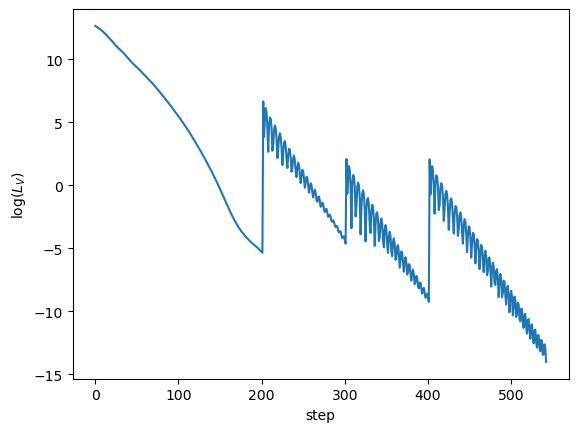
\includegraphics[width=0.5\textwidth]{Figures/loss_cloud_Higgs.png}	\\
	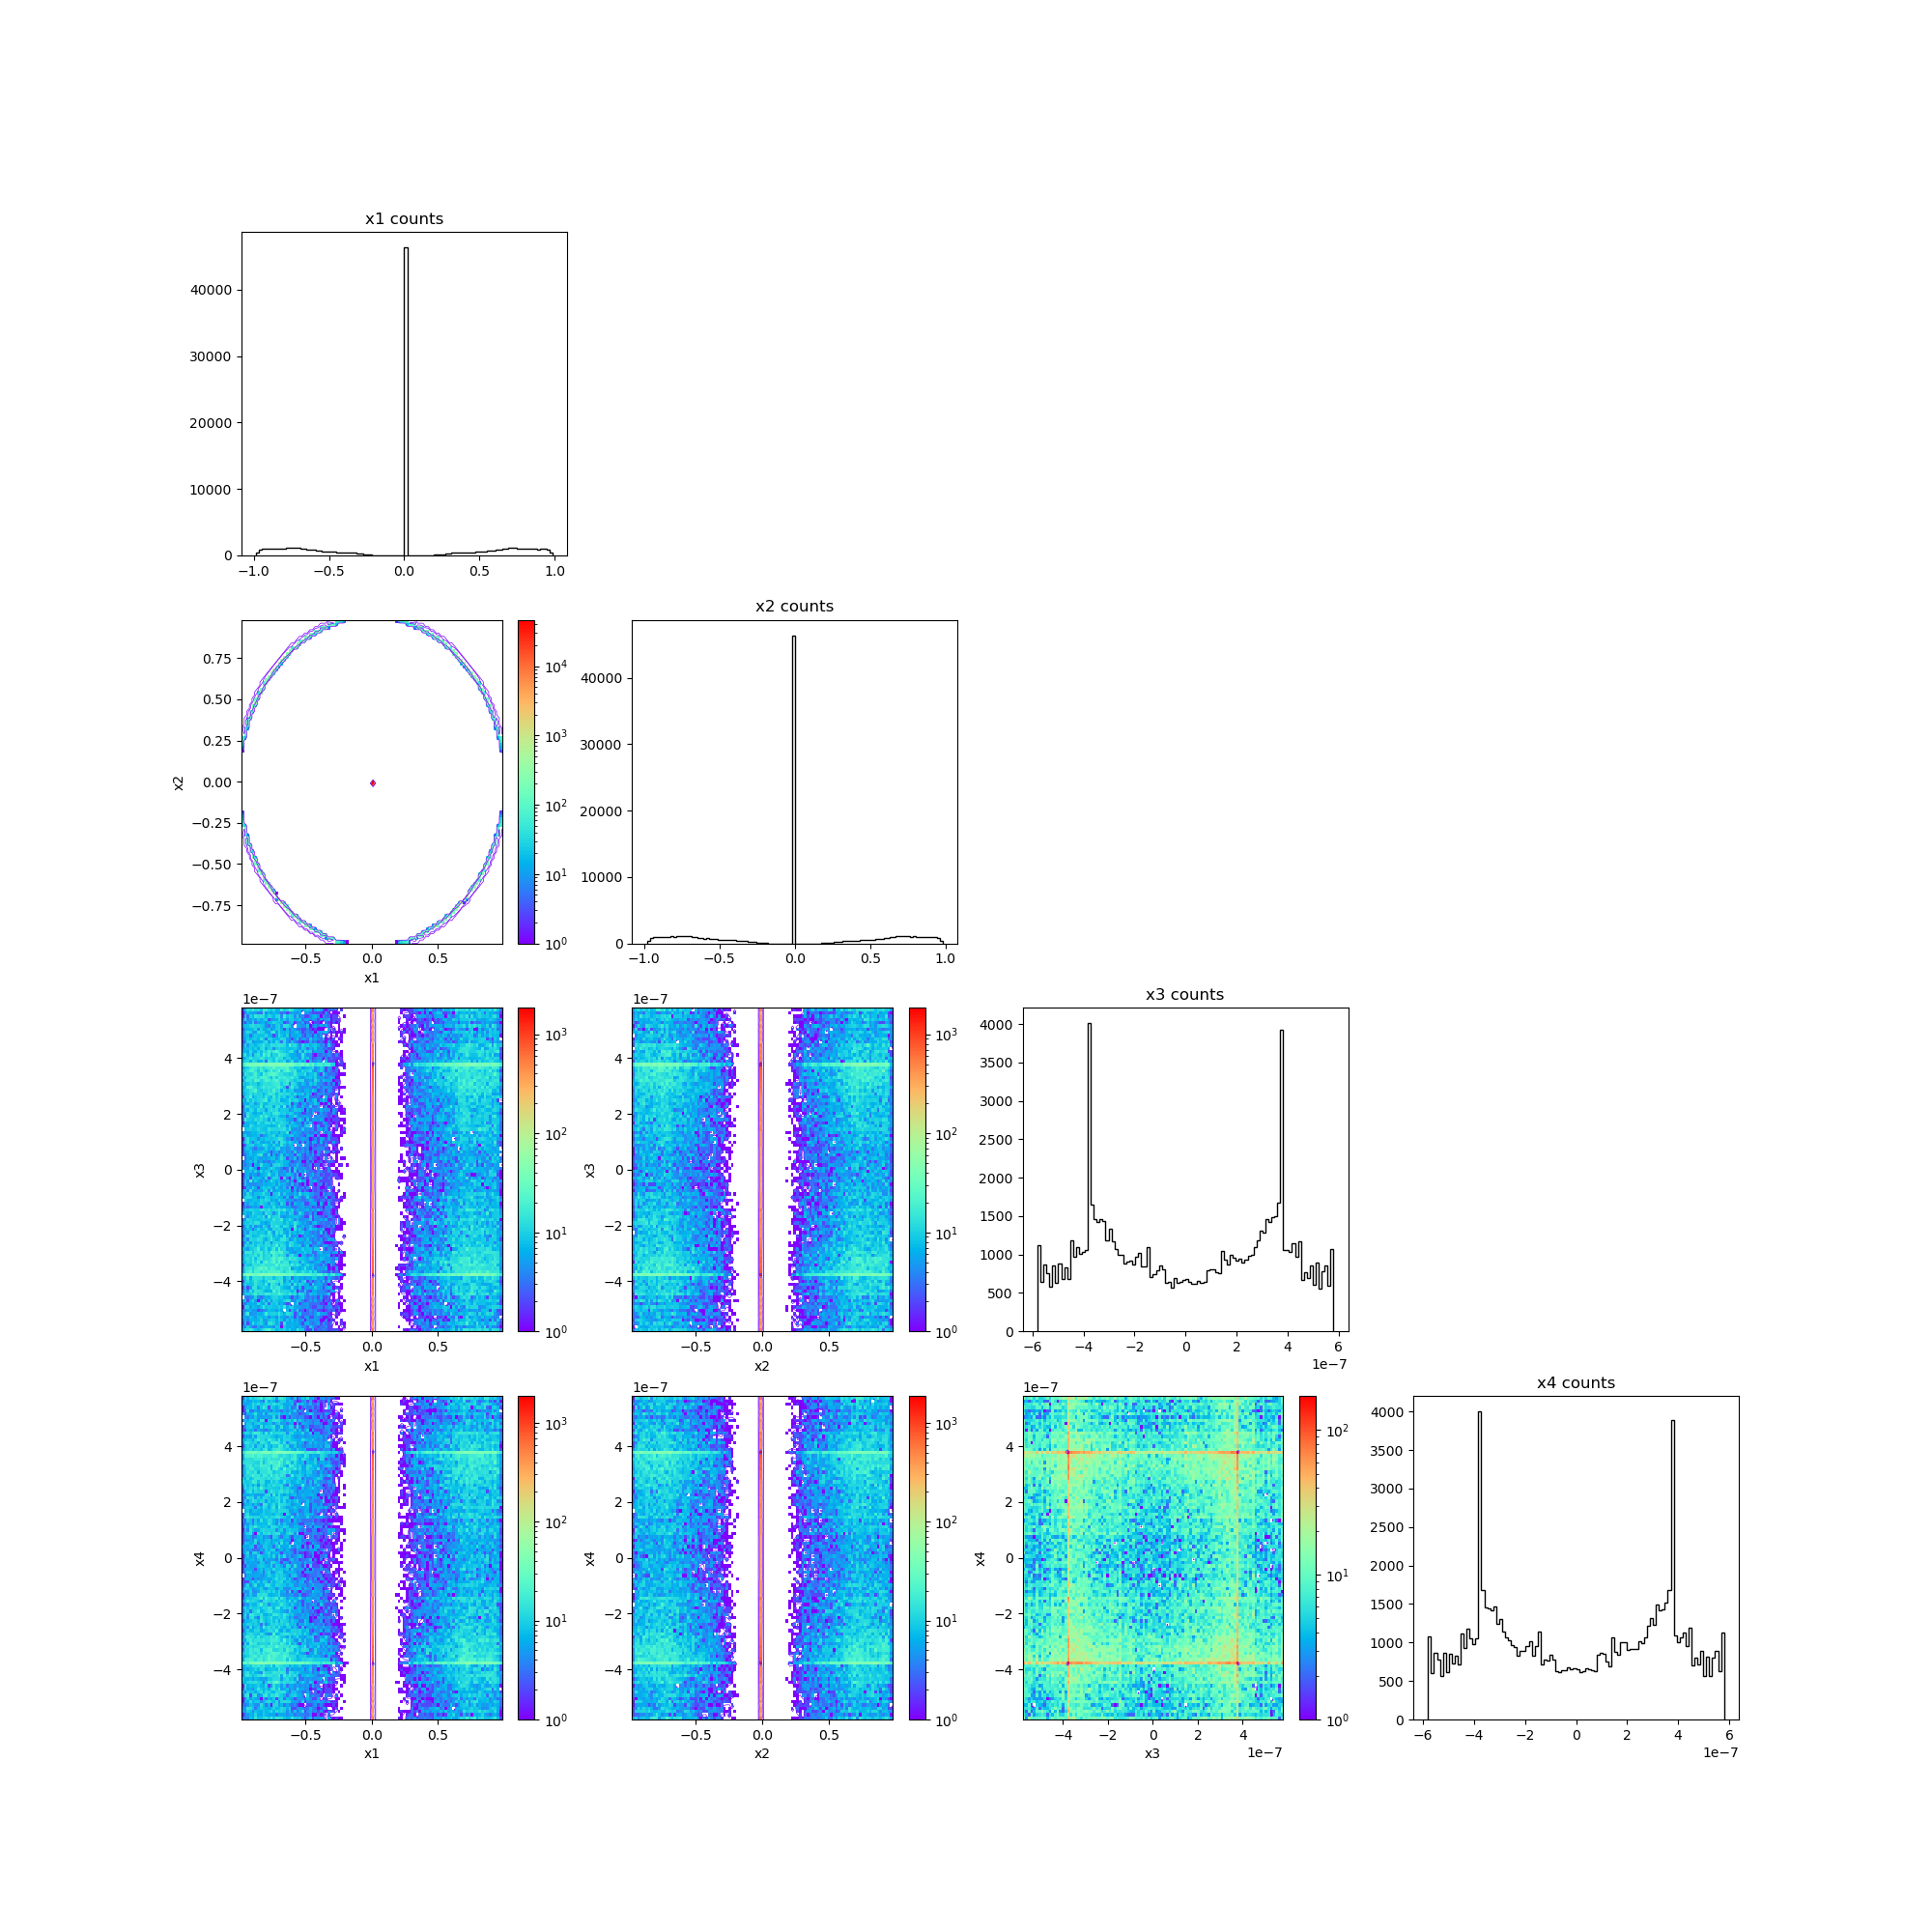
\includegraphics[width=0.85\textwidth]{Figures/triangle_higgs.png}
	\caption{Loss function and triangular plot of the numerical vacua of \eqref{eq:toy1_V}.}
	\label{fig: toy1_cloud}
\end{figure}
%

To ascertain the dimension of the geometric structures behind the shapes in figure~\ref{fig: toy1_cloud}, 
we have employed an AE with the following architectures
%
\begin{equation}	\label{eq: AE_architecture_higgs}
	[n,q_1,q_2,q_3,\ell]=[4,32,16,8,\ell]\,,	\qquad \ell=1,2,3\,,
\end{equation}
%
following the notation of figure~\ref{fig: AE_notation}. For this example, $L_{\rm AE}(\ell)$ in figure~\ref{fig: lossAE_higgs} would naively suggest
that the underpinning structures are two-dimensional, instead of the zero- and one-dimensional loci in \eqref{eq: toy1_CM}.
However, close inspection of the output of the encoder half of the autoencoder \eqref{eq: AE_architecture_higgs} for $\ell=2$ reveals
that the data is cleanly separated into two distinct structures: one point and one (broken) line, as can be observed in 
figure~\ref{fig: encoded_higgs}. In fact, filtering using the decoder to label the data corresponding to the isolated point in
figure~\ref{fig: encoded_higgs}, it can be verified that they correspond to solutions in family 1. Filtering out these points,
the analytical structure of the complementary set can in fact be found to by using the $\ell=1$ decoder as a non-linear function ... 
\note{how were the details of this procedure?}
%

%
\begin{figure}
	\centering
	\subfigure[]{
		\label{fig: lossAE_higgs}	
		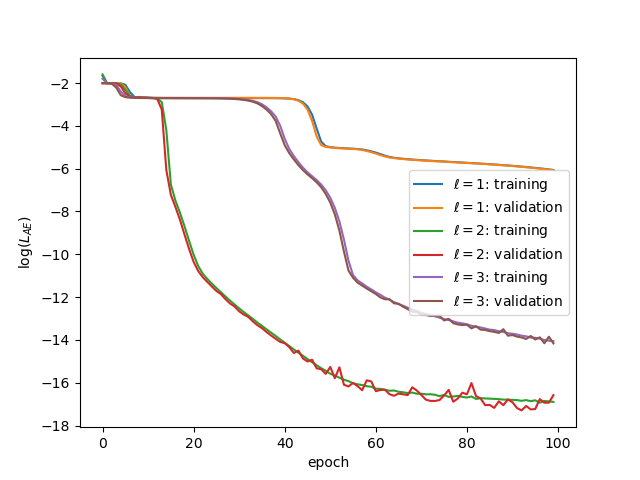
\includegraphics[width=0.48\textwidth]{Figures/lossAE_higgs.png}
	}
	%
	\subfigure[]{
		\label{fig: encoded_higgs}
		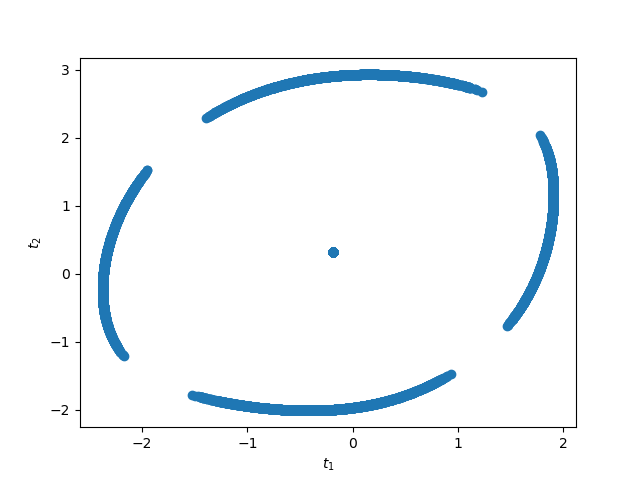
\includegraphics[width=0.48\textwidth]{Figures/encoded_Higgs_l2.png}
	}
	\caption{Loss function encoder output for the autoencoder \eqref{eq: AE_architecture_higgs} and the entire set of data in figure~\ref{fig: toy1_cloud}.}
	\label{fig: AE_higgs}
\end{figure}
%


%%%%%%%%%%%%%%%%%%%%%%%%%
\paragraph{Scrambled Higgs potential}
The example above was somewhat trivial given that one could immediately recognise 
the relevant structure by glancing at figure~\ref{fig: toy1_cloud}, as the variables in which
the solutions in \eqref{eq: toy1_CM} are most naturally expressed coincide with the variables
that appear in the potential. In supergravity this will no longer be the case, and to exemplify
how the autoencoder is useful in this context, let us consider the same potential as above,
%
\begin{equation}	\label{eq:toy2_V}
	V(\tilde{x}^1,\tilde{x}^2,\tilde{x}^3,\tilde{x}^4) = \big[(\tilde{x}^1)^2+(\tilde{x}^2)^2-1\big]^2+(\tilde{x}^3)^2+(\tilde{x}^4)^2\,,
\end{equation}
%
with the variables $\tilde{x}^i$ given by \note{need to decide a non-singular and bijective change of coordinates.}
%
\begin{equation}
	\tilde{x}^1=\dots\,.
\end{equation}
%
Constructing the conformal manifold in terms of $x^i$ results in a could for which the structure of the solutions is
much less clear, as can be appreciated in figure~\ref{fig: toy2_cloud}. 
However, the information in an autoencoder given again by \eqref{eq: AE_architecture_higgs} results in
loss functions and encoded data in precise correspondence with figure~\ref{fig: AE_higgs}.

%%%%%%%%%%%%%%%%
\subsection{SO(8,4) supergravity}

We have

\begin{enumerate}
	\item Looked at 3-, 5-, 7- and 13-parameter truncations.
	\item There was qualitatively different behaviour when using logs vs exps.
	\item There are spurious structures (forks) that the AE erases (why does it?).
	\item The spurious structures can be also be broadened using random walks.
\end{enumerate}



%%%%%%%%%%%%%%%%
\bibliography{references}


\end{document}